\chapter{Tworzenie edytorów graficznych na bazie metamodeli}

Aplikacje komputerowe wykorzystują elementy graficzne aby ułatwić i
przyśpieszyć użytkownikom pracę.
Dzieje się to z uwagi na fakt, że ludzie bardziej efektycznie przyswajają
informacje wizualne (obrazki, diagramy), niż
tekst~\cite{images-more-effective-article}.
W przypadku użytkownika
wpływającego na zachowanie systemu w sposób wizualny (np.\ edytując diagram),
korzysta on wtedy z edytora graficznego i modyfikuje pewien model
rzeczywistości reprezentowany przez program. Model ten zaprojektowany jest
przez twórcę aplikacji i jego struktura również może być reprezentowana na
wiele sposobów. W sytuacji, gdy model został zaprojektowany przez twórcę
aplikacji w środowisku graficznym poprzez narysowanie diagramu jego struktury
mówimy, że ten model modelu to \emph{metamodel}.

\section{Metamodelowanie}

\emph{\Gls{metamodelowanie}} w kontekście wytwarzania oprogramowania to
technika polegająca
na przygotowaniu abstrakcyjnego modelu (metamodelu) opisującego strukturę
modeli, które będą wykorzystywane w programie. Metamodel określa jakie są
dopuszczalne typy obiektów w modelu, ich atrybuty, powiązania między nimi.
Definiuje składnię języka projektowania. Przedrostek \emph{meta} oznacza, że
poziom abstrakcji tego metamodelu jest wyższy niż poziom abstrakcji modelu,
który opisuje.

Wiele powszechnie znanych języków projektowania diagramów ma swoje metamodele
definiujące ich strukturę:

\begin{itemize}
	\item \gls{UML} ma swoją specyfikację~\cite{uml-omg-specification} i
	      metamodel opisany w języku \gls{MOF}.

	\item \gls{BPMN} (język do opisu procesów biznesowych) ma swój
	      metamodel~\cite{bpmn2-metamodel} również opisany w języku \gls{MOF}.

	\item Istnieje artykuł proponujący metamodel dla \gls{ERM}~\cite{entity-relationship-metamodel}. Dla przypomnienia, \gls{ERM} pozwala przedstawić na diagramie encje bazy danych i powiązania między nimi.
\end{itemize}

Aby model był funkcjonalny oprócz jego struktury (składni języka projektowania)
należy zdefiniować i przestrzegać jego semantyki. To ona decyduje o tym jak
należy interpretować model, a także jakie sytuacje, pomimo bycia poprawnymi
strukturalnie, byłyby niewłaściwe z punktu widzenia ich sensowności.

Przykładowo, dla w języku \gls{UML} z perspektywy struktury możliwe jest
utworzenie dwóch klas i dwóch połączeń agregacji między nimi, co zostało
zademonstrowane na rysunku~\ref{rys:nieprawidlowy-model-uml}. Taki model jest
semantycznie niepoprawny, ponieważ relacja kompozycji oznacza, że jeden obiekt
jest zawarty w drugim obiekcie. Oznaczałoby to, że zarówno osoba
(\emph{Person}) jest zawarta w obiekcie samochodu (\emph{Car}) jako jego
właściciel, jak i samochody są zawarte w obiekcie właściciela.

\begin{figure}[!hb]
	\centering

	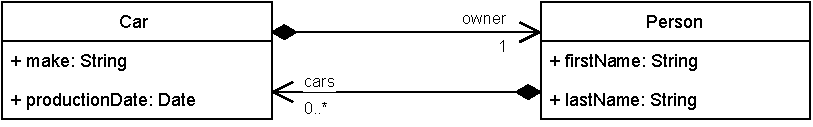
\includegraphics[width=0.95\linewidth]{./images/invalid-uml-example.pdf}
	\caption{Przykład modelu \gls{UML} nieprawidłowego semantycznie.
		Samochód jest jednocześnie częścią osoby, a osoba jest zawarta
		w samochodzie.
	}\label{rys:nieprawidlowy-model-uml}
\end{figure}

Dopiero znając znaczenie relacji kompozycji można zauważyć ten błąd semantyczny
i go poprawić, na przykład jak na rysunku~\ref{rys:prawidlowy-model-uml}. Na
tym diagramie to osoba (\emph{Person}) jest obiektem nadrzędnym, który może
zawierać w sobie odniesienia do samochodów (\emph{Car}). Taki diagram jest
poprawny zarówno składniowo, jak i semantycznie.

\begin{figure}[!hb]
	\centering

	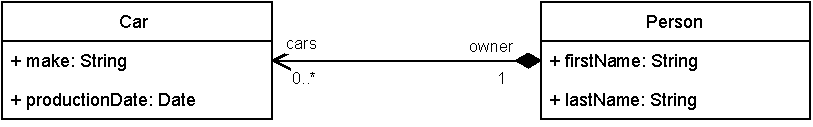
\includegraphics[width=0.95\linewidth]{./images/valid-uml-example.pdf}
	\caption{Przykład prawidłowego modelu
		\gls{UML}. Samochody są tutaj reprezentowane jako części
		obiektu
		\emph{Person} i nie mogą istnieć samodzielnie w
		programie.}\label{rys:prawidlowy-model-uml}
\end{figure}

\section{Edytory graficzne na podstawie metamodeli}
